% Bolo Khata pitch deck. Build: xelatex pitch.tex (run twice).
\documentclass[aspectratio=169,10pt]{beamer}

\usepackage{fontspec}
\usepackage{tikz}
\usetikzlibrary{positioning,arrows.meta,shapes.misc}
\usepackage[most]{tcolorbox}
\usepackage{booktabs}
\usepackage{array}

% ---------- Look: same tokens as app/globals.css ----------
\definecolor{paper}{HTML}{F7F3EC}
\definecolor{card}{HTML}{FFFFFF}
\definecolor{ink}{HTML}{1C1917}
\definecolor{muted}{HTML}{78716C}
\definecolor{line}{HTML}{E7E0D5}
\definecolor{credit}{HTML}{B45309}
\definecolor{creditsoft}{HTML}{FDF1DC}
\definecolor{payment}{HTML}{157347}
\definecolor{paymentsoft}{HTML}{E3F4EA}
\definecolor{amberlite}{HTML}{F6C87A}
\definecolor{greenlite}{HTML}{8FD9AE}

\setsansfont{Segoe UI}
\setmonofont{Consolas}[Scale=0.92]
\usepackage{ragged2e}
\setbeamertemplate{itemize/enumerate body begin}{\RaggedRight}
\tcbset{halign=flush left}
\newfontfamily\deva{Nirmala UI}[Script=Devanagari]
\newfontfamily\semibold{Segoe UI Semibold}
\newcommand{\rs}{{\deva ₹}}

\setbeamercolor{background canvas}{bg=paper}
\setbeamercolor{normal text}{fg=ink}
\setbeamercolor{frametitle}{fg=ink}
\setbeamercolor{itemize item}{fg=credit}
\setbeamercolor{itemize subitem}{fg=muted}
\setbeamertemplate{navigation symbols}{}
\setbeamertemplate{itemize item}{\raisebox{0.15em}{\tikz\fill[credit] (0,0) circle (0.09em);}}
\setbeamertemplate{itemize subitem}{--}
\setbeamersize{text margin left=1.4cm,text margin right=1.4cm}

\setbeamertemplate{frametitle}{%
  \vspace*{0.7cm}%
  {\color{muted}\footnotesize\insertframesubtitle\par}\vspace{2pt}%
  {\semibold\LARGE\insertframetitle\par}%
}
\setbeamertemplate{footline}{%
  \hspace*{1.4cm}{\color{muted}\scriptsize Bolo Khata\hfill\insertframenumber\hspace*{1.4cm}}\vspace*{0.5cm}%
}

% Rounded cards like the app's.
\newtcolorbox{appcard}[1][]{enhanced,colback=card,colframe=line,boxrule=0.6pt,arc=10pt,
  left=10pt,right=10pt,top=8pt,bottom=8pt,#1}
\newtcolorbox{inkcard}[1][]{enhanced,colback=ink,colframe=ink,arc=10pt,coltext=paper,
  left=10pt,right=10pt,top=8pt,bottom=8pt,#1}
\newtcolorbox{creditcard}[1][]{enhanced,colback=creditsoft,colframe=credit,boxrule=0.6pt,arc=8pt,
  left=8pt,right=8pt,top=5pt,bottom=5pt,#1}

\newcommand{\stat}[2]{\begin{appcard}[height=1.6cm,valign=center,halign=center]{\semibold\fontsize{20}{22}\selectfont\color{#1}#2}\end{appcard}}
\newcommand{\lbl}[1]{{\color{muted}\footnotesize #1}}

\begin{document}

% ======================================================================
\begin{frame}[plain]
  \vspace*{1.2cm}
  \begin{columns}[T]
    \begin{column}{0.56\textwidth}
      {\color{muted}\small Sarvam AI hackathon · 2026}\par\vspace{6pt}
      {\semibold\fontsize{40}{44}\selectfont Bolo Khata}\par\vspace{8pt}
      {\Large Speak it. The khata writes itself.}\par\vspace{4pt}
      {\deva\large\color{muted} बोलो, और खाता लिख गया।}\par\vspace{18pt}
      {\small A voice-first credit ledger for India's small shops,\\ built on Sarvam's Indic speech and language models.}\par\vspace{18pt}
      {\scriptsize\color{muted}
      Live\enspace\texttt{bolo-khata-pi.vercel.app}\\[2pt]
      Code\enspace\texttt{github.com/DevVaradPatil/bolo\_khata\_saravam\_ai}}
    \end{column}
    \begin{column}{0.36\textwidth}
      \begin{inkcard}
        {\footnotesize\color{paper!70} Owed to you · {\deva कुल बाकी}}\par
        {\semibold\fontsize{28}{30}\selectfont \rs4,290}\par\vspace{6pt}
        \begin{tcbraster}[raster columns=2,raster equal height,raster column skip=5pt]
          \begin{tcolorbox}[colback=paper!12!ink,colframe=paper!12!ink,arc=6pt,left=5pt,right=5pt,top=3pt,bottom=3pt]
            {\tiny\color{paper!70} Udhaar today}\par{\semibold\color{amberlite}\rs180}
          \end{tcolorbox}
          \begin{tcolorbox}[colback=paper!12!ink,colframe=paper!12!ink,arc=6pt,left=5pt,right=5pt,top=3pt,bottom=3pt]
            {\tiny\color{paper!70} Collected}\par{\semibold\color{greenlite}\rs1,000}
          \end{tcolorbox}
        \end{tcbraster}
      \end{inkcard}
      \vspace{-2pt}
      \begin{creditcard}
        {\footnotesize\semibold Ramesh Dairy · Udhaar \hfill \rs350}
      \end{creditcard}
    \end{column}
  \end{columns}
\end{frame}

% ======================================================================
\begin{frame}{The khata is still on paper}{The problem}
  \begin{columns}[T]
    \begin{column}{0.55\textwidth}
      \begin{itemize}\setlength{\itemsep}{6pt}\small
        \item Neighbourhood shops run on \textbf{udhaar}: regular customers take goods now and pay later.
        \item That credit lives in a paper notebook. Entries get missed, totals drift, and pages get lost.
        \item Ledger apps exist, but they expect \textbf{typing in English} with one hand, at a busy counter.
        \item Owners think and talk in Hindi, Marathi, Hinglish… and in spoken numbers like {\deva ढाई सौ}.
      \end{itemize}
    \end{column}
    \begin{column}{0.36\textwidth}
      \begin{appcard}
        {\lbl{What the owner actually says}}\par\vspace{6pt}
        {\deva “रमेश डेयरी वाले को साढ़े तीन सौ का उधार लिखो, दूध और पनीर।”}\par\vspace{8pt}
        {\lbl{What today's apps need}}\par\vspace{2pt}
        {\small Open app → find customer → tap credit → type 350 → type note → save}
      \end{appcard}
    \end{column}
  \end{columns}
\end{frame}

% ======================================================================
\begin{frame}{Speak. Confirm. Done.}{The solution}
  \centering
  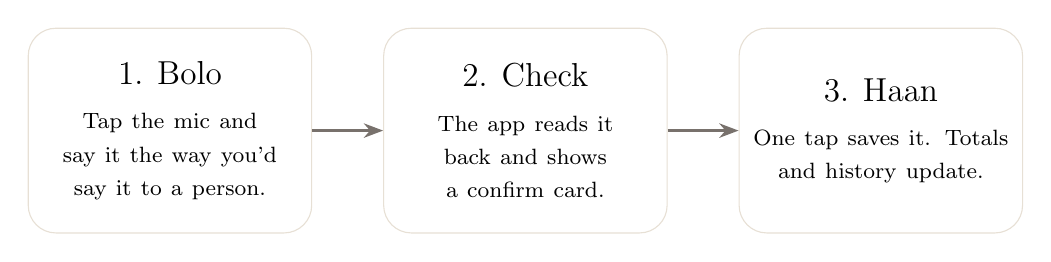
\begin{tikzpicture}[
      stage/.style={rounded corners=10pt,draw=line,fill=card,minimum width=3.6cm,minimum height=2.6cm,align=center,text width=3.3cm},
      arr/.style={-{Stealth[length=7pt]},thick,color=muted}]
    \node[stage] (a) {{\semibold\large 1. Bolo}\\[4pt]{\footnotesize Tap the mic and say it the way you'd say it to a person.}};
    \node[stage,right=0.9cm of a] (b) {{\semibold\large 2. Check}\\[4pt]{\footnotesize The app reads it back and shows a confirm card.}};
    \node[stage,right=0.9cm of b] (c) {{\semibold\large 3. Haan}\\[4pt]{\footnotesize One tap saves it. Totals and history update.}};
    \draw[arr] (a) -- (b); \draw[arr] (b) -- (c);
  \end{tikzpicture}

  \vspace{14pt}
  \begin{minipage}{0.86\textwidth}
    \begin{appcard}
      {\small\color{muted}\deva “सुनीता ताईंनी हजार रुपये दिले”}\hfill{\lbl{Marathi in}}\par\vspace{4pt}
      {\semibold\deva सुनीता पाटिल यांच्याकडून \rs1,000 जमा लिहू का?}\hfill{\lbl{spoken reply out}}
    \end{appcard}
  \end{minipage}

  \vspace{4pt}
  {\footnotesize\color{muted} Also: “Priya ka kitna baaki?” · “Aaj kitna udhaar gaya?” · “Naya customer jodo…” · “Last entry cancel karo”}
\end{frame}

% ======================================================================
\begin{frame}{Every AI step is a Sarvam model}{How it works}
  \centering
  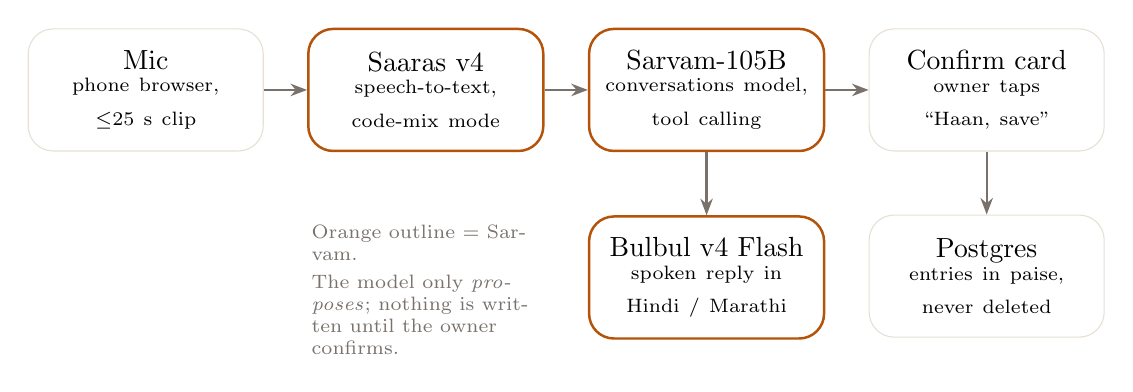
\begin{tikzpicture}[
      box/.style={rounded corners=9pt,draw=line,fill=card,minimum height=1.55cm,text width=2.75cm,align=center},
      sar/.style={box,draw=credit,line width=0.9pt},
      arr/.style={-{Stealth[length=6pt]},thick,color=muted}]
    \node[box] (mic) {{\semibold Mic}\\{\scriptsize phone browser,\\ $\le$25 s clip}};
    \node[sar,right=0.55cm of mic] (stt) {{\semibold Saaras v4}\\{\scriptsize speech-to-text,\\ code-mix mode}};
    \node[sar,right=0.55cm of stt] (llm) {{\semibold Sarvam-105B}\\{\scriptsize conversations model,\\ tool calling}};
    \node[box,right=0.55cm of llm] (card) {{\semibold Confirm card}\\{\scriptsize owner taps\\ “Haan, save”}};
    \node[box,below=0.8cm of card] (db) {{\semibold Postgres}\\{\scriptsize entries in paise,\\ never deleted}};
    \node[sar,below=0.8cm of llm] (tts) {{\semibold Bulbul v4 Flash}\\{\scriptsize spoken reply in\\ Hindi / Marathi}};
    \draw[arr] (mic) -- (stt); \draw[arr] (stt) -- (llm); \draw[arr] (llm) -- (card);
    \draw[arr] (card) -- (db); \draw[arr] (llm) -- (tts);
    \node[below=0.8cm of stt,text width=2.9cm,align=left,font=\scriptsize,color=muted] {
      Orange outline = Sarvam.\\[2pt] The model only \emph{proposes}; nothing is written until the owner confirms.};
  \end{tikzpicture}
\end{frame}

% ======================================================================
\begin{frame}{An agent that knows when to ask}{Agentic design}
  \begin{columns}[T]
    \begin{column}{0.5\textwidth}
      \lbl{Tools the model can call}\par\vspace{4pt}
      \begin{appcard}
        \small
        \texttt{propose\_entry}\hfill{\color{muted}credit / payment}\\
        \texttt{propose\_customer}\hfill{\color{muted}new customer}\\
        \texttt{propose\_undo}\hfill{\color{muted}cancel last entry}\\
        \texttt{get\_balance}\hfill{\color{muted}one customer}\\
        \texttt{list\_dues}\hfill{\color{muted}who owes most}\\
        \texttt{get\_summary}\hfill{\color{muted}today's totals}
      \end{appcard}
      {\footnotesize\color{muted} Several transactions in one sentence become several cards.}
    \end{column}
    \begin{column}{0.42\textwidth}
      \lbl{Two customers called Ramesh}\par\vspace{4pt}
      \begin{appcard}
        {\deva “रमेश को 200 का उधार लिखो”}\par\vspace{6pt}
        {\semibold\deva रमेश कुमार या रमेश डेयरी, कौन से?}\par\vspace{6pt}
        {\footnotesize\color{muted} No guess, no card, nothing saved.}
      \end{appcard}
      \vspace{2pt}
      {\footnotesize Prompt wording alone failed both ways (guessed, or asked “which Ganesh?”). Fix: the \textbf{code} works out shared first names from the database and hands the list to the model.}
    \end{column}
  \end{columns}
\end{frame}

% ======================================================================
\begin{frame}{We measured before we built}{Phase 0 model spike}
  \begin{columns}[T]
    \begin{column}{0.27\textwidth}
      \stat{payment}{15 / 15}
      \centering\lbl{tool calls correct,\\ Hindi · Marathi · Hinglish}
    \end{column}
    \begin{column}{0.27\textwidth}
      \stat{ink}{0.25 s}
      \centering\lbl{per agent reply with\\ sarvam-105b-conversations}
    \end{column}
    \begin{column}{0.27\textwidth}
      \stat{credit}{\rs0.35}
      \centering\lbl{est. cost of one voice turn\\ (STT + LLM + TTS)}
    \end{column}
  \end{columns}
  \vspace{6pt}
  \begin{appcard}[top=5pt,bottom=5pt]
    \footnotesize
    \begin{tabular}{@{}p{4.4cm}p{1.8cm}p{1.8cm}p{4.2cm}@{}}
      \lbl{Chat model} & \lbl{Correct} & \lbl{Avg. reply} & \lbl{Note} \\[2pt]
      \texttt{sarvam-105b} & 14 / 15 & 2.5 s & once wrote a call as text \\
      \texttt{sarvam-105b-conversations} & \textbf{15 / 15} & \textbf{0.25 s} & chosen \\
    \end{tabular}
  \end{appcard}
  {\scriptsize\color{muted} Also found: Saaras keyterm hints turned “Ganesh Kale” into “Ramesh Kale”, so the agent matches names instead.}
\end{frame}

% ======================================================================
\begin{frame}{Built to be trusted with money}{Product}
  \begin{columns}[T]
    \begin{column}{0.48\textwidth}
      \begin{itemize}\setlength{\itemsep}{3pt}\small
        \item \textbf{Confirm before save.} Every change is a card and a spoken read-back.
        \item \textbf{Nothing is deleted.} Undo crosses an entry out; history stays complete.
        \item \textbf{Exact money.} Amounts are stored as whole paise, never decimals.
        \item \textbf{Server re-checks everything} the browser sends back.
        \item \textbf{Bilingual by design.} Names in both scripts; search “Ramesh” or “{\deva सुनीता}”.
        \item \textbf{Typing fallback} for a noisy counter.
      \end{itemize}
    \end{column}
    \begin{column}{0.4\textwidth}
      \begin{appcard}
        {\semibold Ramesh Dairy}\par{\color{muted}\deva रमेश डेयरी}\par\vspace{6pt}
        {\lbl{Owes you}}\par{\semibold\fontsize{24}{26}\selectfont\color{credit}\rs400}
      \end{appcard}
      \vspace{-4pt}
      \begin{appcard}
        \small
        Jama · UPI \hfill {\color{payment}\semibold −\rs150}\\[-1pt]
        {\scriptsize\color{muted} Today, 10:20 pm · Cancelled}\\[3pt]
        Udhaar · Doodh \hfill {\color{credit}\semibold +\rs400}\\[-1pt]
        {\scriptsize\color{muted} 20 Oct}
      \end{appcard}
    \end{column}
  \end{columns}
\end{frame}

% ======================================================================
\begin{frame}{Shipped, live, and small}{Tech}
  \begin{columns}[T]
    \begin{column}{0.46\textwidth}
      \begin{appcard}
        \small
        \lbl{Stack}\par\vspace{3pt}
        Next.js 16 (App Router, streaming) on Vercel\\
        Neon Postgres via Vercel Marketplace\\
        Drizzle ORM · \texttt{pg} connection pool\\
        Sarvam JS SDK \texttt{sarvamai}
      \end{appcard}
    \end{column}
    \begin{column}{0.46\textwidth}
      \begin{appcard}
        \small
        \lbl{Sarvam APIs in use}\par\vspace{3pt}
        \texttt{/speech-to-text} · Saaras v4, codemix\\
        \texttt{/v1/chat/completions} · tools\\
        \texttt{/text-to-speech} · Bulbul v4 Flash\\
        {\color{muted}Next: Mayura translate, Sarvam Vision}
      \end{appcard}
    \end{column}
  \end{columns}
  \vspace{10pt}
  {\small One voice turn today: \textbf{2–5 s} end to end. The biggest pieces are the spoken reply (Bulbul) and the database sitting in the US while users and functions are in India; both have straightforward fixes on the roadmap.}
\end{frame}

% ======================================================================
\begin{frame}{What's next}{Roadmap}
  \begin{columns}[T]
    \begin{column}{0.3\textwidth}
      \begin{appcard}[height=4.3cm]
        {\semibold Reminders}\par\vspace{4pt}
        \small Payment reminder written by \textbf{Mayura} in the \emph{customer's} language, plus a \textbf{Bulbul} voice note, sent on WhatsApp.
      \end{appcard}
    \end{column}
    \begin{column}{0.3\textwidth}
      \begin{appcard}[height=4.3cm]
        {\semibold Scan the old khata}\par\vspace{4pt}
        \small Photograph a paper page. \textbf{Sarvam Vision} extracts name, amount and date rows to review and import.
      \end{appcard}
    \end{column}
    \begin{column}{0.3\textwidth}
      \begin{appcard}[height=4.3cm]
        {\semibold Faster \& multi-shop}\par\vspace{4pt}
        \small Show the transcript first and stream the voice reply; move the database to India; PIN login per shop; “Aaj ka hisaab” daily summary.
      \end{appcard}
    \end{column}
  \end{columns}
\end{frame}

% ======================================================================
\begin{frame}[plain]
  \vspace*{2.2cm}
  \centering
  {\semibold\fontsize{34}{38}\selectfont Bolo Khata}\par\vspace{6pt}
  {\deva\Large\color{muted} बोलो, और खाता लिख गया।}\par\vspace{22pt}
  \begin{minipage}{0.78\textwidth}
    \begin{inkcard}[halign=center]
      \small
      Try it\enspace\texttt{bolo-khata-pi.vercel.app}\\[3pt]
      Code\enspace\texttt{github.com/DevVaradPatil/bolo\_khata\_saravam\_ai}
    \end{inkcard}
  \end{minipage}\par\vspace{10pt}
  {\footnotesize\color{muted} Powered by Sarvam AI · Saaras · Sarvam-105B · Bulbul}
\end{frame}

\end{document}
